%****************************************************
%	CHAPTER 3 - Dynamics
%****************************************************
\chapter{Kinematics \& Dynamics}
\label{ch:dynamics}
%====================================================
Generally applicable rigid body dynamics are first derived. Thereafter, those dynamics are adapted to the non-linear multibody case where constrained relative internal rotational in permitted. Following that, aerodynamic effects are investigated and incorporated into the plant's model. Finally a consolidated, quaternion based plant model is presented which is used for the later control plant development next in Chapter:\ref{ch:control}.
%====================================================
\section{Rigid Body Dynamics}
\label{sec:dynamics.rigidbody}
%====================================================
\subsection{Lagrange Derivation}
\label{subsec:dynamics.rigidbody.lagrange}
%====================================================
Fundamentally any body, rigid or otherwise, can undergo two kinds of movements, namely rotational and translation motions. Often a Lagrangian\cite{classicaldynamics,rotationrigidbody} approach for combined angular and translational movements is used to derive the differential equations of motion for each degree of freedom. The Lagrangian principle ensures that (translational and rotational) kinematic energies and potential energy are conserved throughout the system's trajectory progression. When combined with Euler-Rotational equations, the Euler-Lagrangian\cite{lagrange-formalism} formulation fully defines the aerospace 6-DOF equation set.
\par
Lagrangian formalism is regarded as especially useful in non-cartesian (\emph{spherical etc\ldots}) co-ordinate frames or multi-body systems. With that being said, a cartesian co-ordinate system was already defined in Section:\ref{subsec:proto.conventions.motoraxis}. Rigid body dynamics in a cartesian co-ordinate frame do lend themselves to Newtonian mechanics. The Newton-Euler or Euler-Lagrange formulations both stipulate the same resultant differential equations of motion. The Lagrangian operator, $\mathcal{L}$, is a term consisting of the difference between kinetic and potential energies, $T$ and $U$ respectively. Considering some generalized path co-ordinates $\mathbf{r}(t)$, for both linear $\vec{\mathcal{E}}$ and angular $\vec{\eta}$ relative positions;
\begin{equation}\label{eq:generalpath}
\mathbf{r}(t)=\begin{bmatrix}
\vec{\mathcal{E}} \\
\vec{\eta}
\end{bmatrix}
\end{equation}
The co-ordinates in Eq:\ref{eq:generalpath} are generalized here, despite being symbols commonly used to represent linear and angular positions. The generalized co-ordinates are later be refined as Cartesian body co-ordinates with respect to the inertial frame. The Lagrangian is, by definition:
\begin{subequations}
\begin{equation}\label{eq:lagrangian.a}
\mathcal{L}(\mathbf{r},\dot{\mathbf{r}},t)=T(\mathbf{r},\dot{\mathbf{r}})-U(\mathbf{r},\dot{\mathbf{r}})
\end{equation}
With kinetic and potential energy function(s) $T$ and $U$ respectively. Then introducing a rigid body's general kinetic (angular \& linear) and potential energies, in some shared reference frame. In this case the only potential energy is gravitational\footnote{Here $G=\begin{bmatrix}
0&0&-9.81
\end{bmatrix}^T~m.s^{-2}$~in the Inertial frame,$\in\mathcal{F}^I$} potential energy:
\begin{equation}\label{eq:lagrangian.b}
\mathcal{L}=
\frac{1}{2}
\begin{bmatrix}
\dot{\vec{\mathcal{E}}}^{~T}(m)\dot{\vec{\mathcal{E}}}\\
\dot{\vec{\eta}}^{~T}(\mathbb{I}_b)\dot{\vec{\eta}}
\end{bmatrix}
-
\begin{bmatrix}
m\vec{G}z\\
0
\end{bmatrix}
\end{equation}
\end{subequations}
Noting that $\mathbb{I}_b$ is the inertial tensor of the body aligned w.r.t to whichever reference frame is used. The Euler-Lagrange formulation equates partial derivatives of the Lagrangian to any generalized forces, $\mathbf{V}$, acting on the system. In this case the generalized forces or, more specifically a net force $\vec{F}_{net}$ and a net torque $\vec{\tau}_{net}$.
\begin{equation}\label{eq:euler-lagrange}
\frac{d}{dt}\bigg(\frac{\delta L}{\delta \dot{\mathbf{r}}}\bigg)-\frac{\delta L}{\delta \mathbf{r}} = \mathbf{V} = \begin{bmatrix}
\vec{F}_{net}\\
\vec{\tau}_{net}
\end{bmatrix}
\end{equation}
And taking the partial derivatives of Eq:\ref{eq:lagrangian.b} with respect to the path co-ordinates $\mathbf{r}$:
\begin{subequations}
\begin{equation}\label{eq:partial.a}
\frac{\delta L}{\delta \mathbf{r}}=\begin{bmatrix}
m\vec{G}_x\\
0
\end{bmatrix}
\end{equation}
\vspace{-5pt}
\begin{equation}\label{eq:partial.b}
\frac{d}{dt}\bigg(\frac{\delta L}{\delta \dot{\mathbf{r}}}\bigg)=\bigg[
m\frac{d}{dt}\dot{\vec{\mathcal{E}}} ~~~ \mathbb{I}\frac{d}{dt}\dot{\vec{\eta}}\bigg]^T
\end{equation}
\end{subequations}
Where $\vec{G}_x$ is the gravitation force in whichever reference frame ($\mathcal{F}^x$) the lagrangian is with respect to. In any generalized coordinate system a rotating vector's time derivative which, according to the Reynolds Transportation Theorem\cite{reynolds}, is given by:
\begin{equation}\label{eq:reynolds}
\frac{d\vec{f}}{dt_a}=\frac{d\vec{f}}{dt_b}+\vec{\omega}_{a/b}\times\vec{f}
\end{equation}
So applying that theorem (Eq:\ref{eq:reynolds}) to the partial derivatives in Eq:\ref{eq:partial.b} and further defining the generalized co-ordinates as cartesian body coordinates with respect to an inertial origin (the body frame $\mathcal{F}^b$ and inertial frame $\mathcal{F}^I$). Noting that in Eq:\ref{eq:partial.b} the place holders used for linear ($\vec{\mathcal{E}}$) and angular positions ($\vec{\eta}$) all exist in a common shared frame\footnote{In this case $\vec{\eta}\not=[\phi~\theta~\psi]^T$ seeing that the angular position $\vec{\eta}$ is defined in a common frame. $\vec{\eta}$ is \underline{NOT an Euler angle} set.}, and hence:
\begin{equation}
\frac{d}{dt}
\begin{bmatrix}
{\mathcal{E}}\\
\vec{\eta}
\end{bmatrix}
\triangleq
\begin{bmatrix}
\vec{\nu}\\
\vec{\omega}
\end{bmatrix}
\in \mathcal{F}^b
\end{equation}
It then follows that the Lagrangian Eq:\ref{eq:lagrangian.b} changes to:
\begin{subequations}
\begin{equation}
\mathcal{L}=\frac{1}{2}
\begin{bmatrix}
\vec{\nu}^{~T}(m)\vec{\nu}\\
\vec{\omega}^{~T}(\mathbb{I})\vec{\omega}
\end{bmatrix}
-
\begin{bmatrix}
m\vec{G}_b z\\
0
\end{bmatrix}
\end{equation}
\vspace{-5pt}
\begin{equation}
\frac{d}{dt}\bigg(\frac{\delta L}{\delta \dot{\mathbf{r}}}\bigg)=\bigg[
m\frac{d}{dt}\vec{\nu} ~~~ \mathbb{I}\frac{d}{dt}\vec{\omega}\bigg]^T
\end{equation}
\vspace{-5pt}
\begin{equation}
\rightarrow m\frac{d}{dt}\vec{\nu}=m\dot{\vec{\nu}}+\vec{\omega}_{I/b}\times\vec{\nu}
\end{equation}
\vspace{-5pt}
\begin{equation}
\rightarrow \mathbb{I}_b \frac{d}{dt}\vec{\omega}=\mathbb{I}_b\dot{\vec{\omega}}+\vec{\omega}_{I/b}\times\mathbb{I}_b\vec{\omega}
\end{equation}
\end{subequations}
Which, when substituted back into the Euler-Lagrange formulation Eq:\ref{eq:euler-lagrange}, results in the familiar Newton-Euler equations for linear and angular differentials, both in the body frame;
\begin{subequations}\label{eq:newton}
\begin{equation}\label{eq:newton.a}
\vec{F}_{net}=m\dot{\vec{\nu}}+\vec{\omega}_b\times m \vec{\nu} - m\mathbb{R}_I^b(-\eta) \vec{G}_I
\end{equation}
\vspace{-15pt}
\begin{equation}\label{eq:newton.b}
\vec{\tau}_{net}=\mathbb{I}_b\dot{\vec{\omega}}_b+\vec{\omega}_b\times\mathbb{I}_b\vec{\omega}_b
\end{equation}
\end{subequations}
It's important to recall that $\vec{\omega}_b\not= \dot{\vec{\eta}}$ where $\vec{\eta}=[\phi~\theta~\psi]^T$, seeing that Euler Angles are defined in sequentially rotated reference frames. So then four differential equations are often used to completely describe the entire set of state derivatives, namely:
\begin{subequations}\label{eq:states}
\begin{equation}\label{eq:states.a}
\dot{\vec{\mathcal{E}}}=\mathbb{R}_b^I(-\eta)\vec{\nu}~~~~\in\mathcal{F}^I
\end{equation}
\vspace{-10pt}
\begin{equation}\label{eq:states.b}
\vec{F}_{net}=m\dot{\vec{\nu}}+\vec{\omega}_b\times m\vec{\nu} -m \mathbb{R}_I^b(-\eta)\vec{G}_I ~~~~\in\mathcal{F}^b
\end{equation}
\newpage
\begin{equation}\label{eq:states.c}
\dot{\vec{\eta}}=\Psi(\eta)\vec{\omega}_b~~~~\in\mathcal{F}^{v2},\mathcal{F}^{v1},\mathcal{F}^I
\end{equation}
\vspace{-10pt}
\begin{equation}\label{eq:states.d}
\vec{\tau}_{net}=\mathbb{I}_b\dot{\vec{\omega}}_b+\vec{\omega}_b\times\mathbb{I}_b\vec{\omega}_b~~~~\in\mathcal{F}^b
\end{equation}
\end{subequations}
The state differentials in Eq:\ref{eq:states} can be reduced to a set of two equations. Those differentials are defined in reference frames of the state variables which they represent. The non-linear form of those equations substitutes\footnote{Originally introduced in Eq:\ref{eq:angular-rates.e}} $d\vec{\eta}/dt=\Phi(\eta)\vec{\omega}_b$ in the Lagrangian derivative, Eq:\ref{eq:partial.b}.
\begin{equation}
\frac{d}{dt}\bigg(\frac{\delta \mathcal{L}}{\delta \dot{\mathbf{r}}}\bigg)=\bigg[m\frac{d}{dt}\vec{\nu}~~~\mathbb{I}\frac{d}{dt}\dot{\vec{\eta}}\bigg]^T\Rightarrow\bigg[m\frac{d}{dt}\vec{\nu}~~~\mathbb{I}\frac{d}{dt}\Phi(\eta)\vec{\omega}_b\bigg]^T
\end{equation}
This only affects the angular component as the two kinetic energies are independent of one another. And so applying the differential chain rule:
\begin{equation}
\mathbb{I}\frac{d}{dt}\Phi(\eta)\vec{\omega}_b=\mathbb{I}\big(\Phi\dot{(\eta)}\vec{\omega}_b+\Phi(\eta)\dot{\vec{\omega}}_b \big)
\end{equation}
Drawing from \cite{autonomousrobotseuler} and recognizing that $\mathbb{I}$ must be transformed to the common intermediate Euler axes, $\mathbb{J}=\Psi(\eta)^T\mathbb{I}\Psi(\eta)$. The controllable differential equation for angular acceleration in Eq:\ref{eq:newton.b}, then in intermediate Euler frames for each angle becomes\footnote{The relationship $\dot{\Phi}=\Phi\dot{\Psi}\Phi$ was used to simplify Eq:\ref{eq:nonlinear}, the singularity in $\Phi$ still remains\ldots}:
\begin{subequations}\label{eq:nonlinear}
\begin{equation}\label{eq:nonlinear.a}
M(\eta)\ddot{\vec{\eta}}+C(\eta,\dot{\eta})\dot{\vec{\eta}}=\Psi(\eta)\vec{\tau}_{net}
\end{equation}
\vspace{-15pt}
\begin{equation}\label{eq:nonlinear.b}
M(\eta)=\Psi(\eta)^T\mathbb{I}\Psi(\eta)
\end{equation}
\vspace{-10pt}
\begin{equation}\label{eq:nonlinear.c}
C(\eta,\dot{\eta})=-\Psi(\eta)\mathbb{I}\Psi\dot{(\eta)}+\Psi(\eta)^T \big[\Psi(\eta)\dot{\vec{\eta}}\big]_{\times}\mathbb{I}\Psi(\eta)
\end{equation}
\end{subequations}
Equation \ref{eq:nonlinear.a} fully describes the state derivative $\ddot{\vec{\eta}}$ in its own frame(s). The two differential equations which describe the entire bodies motion are then:
\begin{subequations}
\begin{equation}\label{eq:rigid-frame.a}
\vec{F}_{net}=m\dot{\vec{\mathcal{E}}}+\mathbb{R}_b^I(-\eta)\vec{\omega}_b \times m \dot{\vec{\mathcal{E}}}-m\vec{G}_I~~~~\in\mathcal{F}^I
\end{equation}
\vspace{-10pt}
\begin{equation}\label{eq:rigid-frame.b}
\vec{\tau}_{net}=\Psi(\eta)^{-1}M(\eta)\ddot{\vec{\eta}}+\Psi(\eta)^{-1}C(\eta,\dot{\eta})~~~~\in\mathcal{F}^{v2,v1,I}
\end{equation}
\end{subequations}
\par
The generalized net forces effecting the system, $\vec{F}(u)$ and $\vec{\tau} (u)$, are the system's controllable inputs and are going to be affected directly the systems actuators and their associated effectiveness function. In the general case, which is expanded upon in Section:\ref{sec:dynamics.aero}, the control inputs are typically as follows:
\begin{subequations}
The net force acting on the system is just the sum of all thrust vectors produced by rotating propellers, $T(\Omega_i)$.
\begin{equation}
\mu \vec{F} = \sum_{i=1}^4 \vec{T}(\Omega_i)
\end{equation}
Secondly the net torque is the sum of all torque arms produced from those propeller thrust vectors.
\begin{equation}
\mu \vec{\tau} = \sum_{i=1}^4 \vec{l}_i \times \vec{T}(\Omega_i)
\end{equation}
\end{subequations}
Where $\vec{T}(\Omega_i)$ is the $i^{th}$ motor's thrust vector, not necessarily in $\mathbb{R}^3$, and typically bound to the $\hat{Z}_b$ axis, $\vec{l}_i$ is that thrust vector's perpendicular displacement from the origin $\mathbf{O}_b$. The above equations are still applicable to any 6 DOF body, common simplifications applied to the system(s) for quadrotor control are explored in Appendix:\ref{app:stddynamics}. Aspects unique to (multibody) aerospace frames are now introduced. Obviously the focus is on quadrotor and tilting quadrotor platforms\ldots
%====================================================
\subsection{Rotation Matrix Singularity}\label{subsec:dynamics.rigidbody.singularity}
%====================================================
The Euler Angle singularity is often mentioned but far less common is the demonstration of exactly how that singularity \emph{mathematically} manifests itself. By definition, a singularity occurs when a loss of differentiability is encountered. In the case of an affixed 3-axis gimbal (Fig:\ref{fig:gimbal}), when an intermediary rotational angle, for example the rolling angle $\theta$, is at $\pi/2$ then the remaining two axes become co-linear (Fig:\ref{fig:gimbal-lock}). That being both pitch $\phi$ or yaw $\psi$ rotations will subsequently have the same effect. Such a situation results in what is termed as a loss of a degree of freedom.
\begin{figure}[htbp]
\begin{subfigure}{0.5\textwidth}
\centering
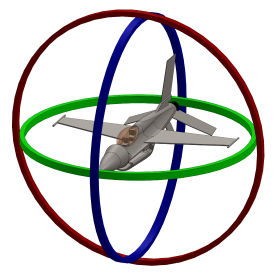
\includegraphics[width=\textwidth]{figs/gimbal}
\caption{3-Axis gimbal}
\label{fig:gimbal}
\end{subfigure}
\begin{subfigure}{0.5\textwidth}
\centering
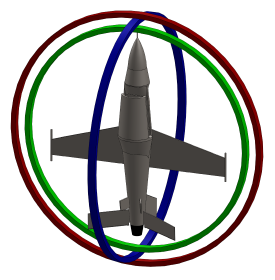
\includegraphics[width=\textwidth]{figs/gimbal-lock}
\caption{Locked gimbal with loss of DOF}
\label{fig:gimbal-lock}
\end{subfigure}
\caption{Gimbal lock}
\end{figure} 
\par
What is clear in a physical system is not necessarily as clear mathematically. An obvious loss of differentiability is manifested in the Euler Matrix $\Psi(\eta)$, Eq:\ref{eq:angular-rates.e} from Section:\ref{subsec:proto.conventions.frames}. The relation between angular velocity, in the inertial frame or inversely in the body frame, and the angular rates of the Euler Angles.
\begin{equation}\label{eq:euler-derivative}
\begin{bmatrix}
\dot{\phi}\\
\dot{\theta}\\
\dot{\psi}
\end{bmatrix}
=\begin{bmatrix}
1 & sin(\phi)tan(\theta) & cos(\phi)tan(\theta)\\
0 & cos(\phi) & -sin(\phi)\\
0 & sin(\phi)sec(\theta) & cos(\phi)sec(\theta)\\
\end{bmatrix}
\begin{bmatrix}
p\\
q\\
r
\end{bmatrix}
=\Phi(\eta)\omega_b
\end{equation}
\begin{equation}
\text{As}~\underset{{\theta \rightarrow \pi /2}}{lim}~sec(\theta),tan(\theta)\rightarrow \infty
\end{equation}
Or that $\Phi(\eta)$ is undefined at $\theta=\pi/2$. 
It's clear to see that in Eq:\ref{eq:euler-derivative} there exists an undefined singularity as $\theta\rightarrow\pi/2$. The physical consequence of this is the loss of a degree of freedom. More specifically, if one looks at how the Z-Y-X rotation (or transformation) matrices are formulated:
\begin{subequations}
\begin{equation}
\mathbb{R}_I^b = \mathbb{R}_z\mathbb{R}_y\mathbb{R}_x=\begin{bmatrix}
c_\psi & -s_\psi & 0\\
s_\psi & c_\psi & 0\\
0 & 0 & 1
\end{bmatrix}
\begin{bmatrix}
c_\theta & 0 & s_\theta\\
0 & 1 & 0\\
-s_\theta & 0 & c_\theta
\end{bmatrix}
\begin{bmatrix}
1 & 0 & 0\\
0 & c_\phi & -s_\phi\\
0 & s_\phi & c_\phi
\end{bmatrix}
\end{equation}
\begin{equation}
\mathbb{R}_I^b=\begin{bmatrix}
c_\psi c_\theta & c_\psi s_\theta s_\phi - s_\psi c_\phi & c_\psi s_\theta c_\phi + s_\psi s_\phi\\
s_\psi c_\theta & s_\psi s_\theta s_\phi + c_\psi c_\phi & s_\psi s_\theta  c_\phi - c_\psi s_\phi\\
-s_\theta & c_\theta s_\phi & c_\phi c_\theta\\
\end{bmatrix}
\end{equation}
In the case where $\theta=\pi/2$, and using trigonometric double angles;
\begin{equation}\label{eq:gimbal}
=\begin{bmatrix}
0 & c_\psi s_\phi - s_\psi c_\phi & c_\psi c_\phi + s_\psi s_\phi\\
0 & s_\psi s_\phi + c_\psi c_\phi & s_\psi c_\phi - c_\psi s_\phi\\
-1 & 0 & 0\\
\end{bmatrix}
=
\begin{bmatrix}
0 & s(\phi - \psi) & c(\phi - \psi)\\
0 & c(\phi - \psi) & s(\phi - \psi)\\
-1 & 0 & 0
\end{bmatrix}=\mathbb{R}_{x'}(\phi-\psi)
\end{equation}
\end{subequations}
Where the resultant in Eq:\ref{eq:gimbal} represents an X-axis rotation in a new intermediate frame, post a $\pi/2$ rotation in the y-axis. Through trigonometric double angles a degree of freedom is lost at $\theta=\pi/2$, when $\phi$ \& $\psi$ effect the same angle.
%====================================================
\subsection{Quaternion Dynamics}
\label{subsec:dynamics.rigidbody.quaternion}
%====================================================
An algorithm proposed in \emph{How To Avoid a Singularity When Using Euler Angles?}\cite{euleranglesingularity} suggested a solution to the problem of Euler Angle singularities. The proposed heuristic was to switch between sequencing conventions (ZYX,ZYZ etc\ldots there are 12 in total) such that the singularity is always avoided. However the implementation of such an algorithm is cumbersome and inefficient. Far more elegant is the use of \emph{quaternion} attitude representations in $\mathbb{R}^4$ (\cite{rotationsequences,quaterniondynamics,spacecraftattitutdequaternions} amongst others\ldots).
\par
A quaternion is analogous to a rotation matrix in that it represents an attitude difference between two reference frames. An $\mathbb{R}^3$ position is paramterized as a single rotation $\theta$ about a unit axis $\hat{u}$ (Sic Rodriguez Formula\cite{unwinding}). Without deliberating too much on their proof or details, a quaternion consists or a scalar component, $q_0$, and complex vector component, $\vec{q}\in \mathbb{C}^3$, such that;
\begin{equation}
Q\triangleq 
\begin{bmatrix}
q_0 \\
\vec{q}
\end{bmatrix}
~~\in\mathbb{R}^4
\end{equation}
The relationship between an Euler Angles rotation matrix $\mathbb{R}_I^b(\eta)$ and a quaternion attitude $Q_b$ is given by the Rodriguez formula:
\begin{equation}\label{eq:rodriguez}
\mathbb{R}_I^b(\eta)=\mathbb{R}(Q_b)=\mathbb{I}+2q_0[\vec{q}~]_\times+2[\vec{q}~]^2_\times
\end{equation}
Any and all quaternions, unless otherwise stated, in this dissertation are all unit quaternions\footnote{Unit quaternions are a subset of the quaternion space}, $Q\in\mathbb{Q}_u$. The need for quaternions with unity magnitude is such to ensure rotational operations don't affect the magnitude of the vector operand. A unit quaternion is defined as:
\begin{equation}
||Q||=\sqrt{{q_0}^2+\vec{q}~^2}=1
\end{equation}
Quaternion multiplication is distributive and associative, but not commutative. Specifically a quaternion multiplciation operation is equivalent to the Hamilton product. For two quaternions, $Q$ \& $P$:
\begin{subequations}
\begin{equation}
Q\otimes P = \begin{bmatrix}
q_0 \\
\vec{q}
\end{bmatrix}
\otimes
\begin{bmatrix}
p_0 \\
\vec{p}
\end{bmatrix}
\end{equation}
\vspace{-5pt}
\begin{equation}
=q_0 p_0 - \vec{q}\cdot \vec{p}+p_0 \vec{q} + q_0 \vec{p} + \vec{q}\times\vec{p}
\end{equation}
\end{subequations}
Seeing that the vector component of a quaternion is complex valued, it is natural that there exists a quaternion conjugate property. Namely:
\begin{equation}
Q^*=\begin{bmatrix}
q_0 \\
-\vec{q}
\end{bmatrix}
\end{equation}
It then follows that\footnote{Disambigation:$\mathbb{I}$ in this context is a $4\times 4$ identity matrix, not an inertial matrix}:
\begin{equation}
Q\otimes Q^* = \mathbb{I}_{4\times 4}
\end{equation}
To apply quaternion rotations to a vector $\vec{v} \in\mathbb{R}^3$ involves multiplication by two unit quaternions. 
\begin{equation}
\begin{bmatrix}
0 \\
\vec{v}~'
\end{bmatrix}
=Q\otimes
\begin{bmatrix}
0 \\
\vec{v}
\end{bmatrix}
\otimes Q^*
\end{equation}
Mostly, the zero scalar components are omitted in a rotation (\emph{or transformation}) operation, such that it is recognized the vector operands are substituted with quaternions.
\begin{equation}\label{eq:quaternion-rotation}
\vec{v}~'=Q \otimes (\vec{v}) \otimes Q^*
\end{equation} 
In the case of rigid body attitude representation, $Q_b$ is the quaternion which represents the difference between $\mathcal{F}^b$ and $\mathcal{F}^I$. A quaternion operator is equivalent to a rotation matrix operation:
\begin{equation}
\mathbb{R}_I^b \underset{Q}{\iff} Q_b \otimes (.) \otimes Q_b^*
\end{equation}
A quaternion time derivative, with $Q_\omega$ being a quaternion with a vector component equal to angular velocity $\omega\in\mathcal{F}^b$ and a zero scalar component, is given by:
\begin{equation}
\frac{d}{dt}Q_b=\frac{1}{2}Q_b\otimes Q_{\omega}=\begin{bmatrix}
-\frac{1}{2}\vec{q}^{~T} \vec{\omega}_b\\
\frac{1}{2}\big([\vec{q}~]_\times+q_0\mathbb{I}\big)\vec{\omega}_b
\end{bmatrix}
\end{equation}
Using quaternions to represent attitudes negates the need for an Euler Matrix, $\Phi(\eta)$, to represent attitudes and their rates. A body quaternion is fully defined in the body frame. The first quaternion time derivative replaces Eq:\ref{eq:states.a}\& Eq:\ref{eq:states.c};
\begin{subequations}
\begin{equation}
\dot{\mathcal{E}}=\mathbb{R}_b^I(-\eta)\vec{\nu}\underset{Q}{\iff}Q_b\otimes\vec{\nu}\otimes Q_b^*
\end{equation}
\vspace{-10pt}
\begin{equation}
\dot{\eta}=\Phi(\eta)\vec{\omega}_b\underset{Q}{\iff}\dot{Q}=\frac{1}{2}Q_b\otimes Q_\omega
\end{equation}
\end{subequations}
Second order derivatives for quaternion acceleration aren't as useful as their velocity counterparts. The second order derivative is mentioned here however it's only relevant to quaternion backstepping in the control chapter. If possible, quaternion accelerations are mostly avoided due to their complexity;
\begin{equation}
\ddot{Q}\big(\dot{Q},Q,t)=\dot{Q}\otimes Q^* \otimes \dot{Q}+\frac{1}{2}Q\otimes \big[\mathbb{I}_b^-1(\tau-4(Q^*\otimes \dot{Q})\times(\mathbb{I}_b(Q^*\otimes \dot{Q}))\big]
\end{equation}
%====================================================
\subsection{Quaternion Unwinding}
\label{subsec:dynamics.rigidbody.unwinding}
%====================================================
Although quaternions are better than Euler angles and lack the associated singularity, they do contain one caveat. Seeing that a quaternion $Q=[q_0~\vec{q}~]^T$ represents an attitude orientation of a body in $\mathbb{R}^3$ using $\mathbb{R}^4$ variables there exists what is called dual coverage\cite{unwinding}.
Each unit quaternion, stemming from Euler-Rodriguez theorem, is parametrized such that the quaternion operation represents an eigenaxis rotation of $\theta$ about an axis $\hat{u}$ such that:
\begin{equation}
Q=\begin{bmatrix}
q_0\\
\vec{q}
\end{bmatrix}=
\begin{bmatrix}
cos(\theta/2)\\
sin(\theta/2)\hat{u}
\end{bmatrix}
\end{equation}
That rotation is executed through the quaternion operator Eq:\ref{eq:quaternion-rotation}. As a result its clear to see that for each unique attitude in 3-Dimensions there exist two quaternions which correlate to the same position. Namely:
\begin{subequations}
\begin{equation}
Q =
\begin{bmatrix}
q_0 \\
\vec{q}
\end{bmatrix}
=
\begin{bmatrix}
cos(\theta/2)\\
sin(\theta/2)\hat{u}
\end{bmatrix}
.
\end{equation}
And seeing that $\theta=2\pi-\theta$, then;
\begin{equation}
Q=\begin{bmatrix}
cos(\pi - \theta/2)\\
sin(\pi - \theta/2)\hat{u}
\end{bmatrix}
=
\begin{bmatrix}
-cos(\theta/2)\\
sin(\theta/2)\hat{u}
\end{bmatrix}
\end{equation}
\end{subequations}
Every physical attitude in $\mathbb{R}^3$ has two corresponding quaternions in $\mathbb{R}^4$; $[\pm q_0~\vec{q}~]^T$. A consequence of this is two possible error state trajectories for every attitude difference. A clockwise $\theta$ rotation and an anticlockwise $2\pi-\theta$ negative rotation. This could lead to an erroneous and unnecessary "unwinding" of a complete counter revolution as a result of a dual covered error state. 
\par
Often the sign scalar component of the attitude quaternion error (Section:\ref{subsec:control.attitude.quaternion}) is simply neglected or assumed positive. As such for attitude controllers the requirement is that for positive and negative scalars the control input is consistent:
\begin{equation}
\nu_d=h([q_0~\vec{q}~]^T,t)=h([-q_0~\vec{q}~]^T,t)
\end{equation}
Or more simply that $Q_e=[|q_0|~\vec{q}~]^T$. The most simple solution which adheres to that constraint is to simply neglect the scalar component and use $h(\vec{q}_e,t)$. A positive quaternion scalar will always ensure that an error state represents a right-handed clockwise rotation. If the resolution of trajectory co-ordinates generated is sufficiently high enough, the control plant will never encounter a problem.
\par
One proposal in \emph{Nonlinear Quadcopter Attitude Control}\cite{nonlinearquadcopter} suggested using a \emph{signum} operator to design the signs of the controller coefficients for the virtual control plant input. 
\begin{subequations}\label{eq:signum-unwinging}
\begin{equation}
\vec{\omega}_d=\frac{2}{\tau}sgn(q_0)\vec{q}
\end{equation}
\vspace{-10pt}
\begin{equation}
sgn(\vec{q})=
\begin{cases}\begin{array}{ll}
1 & ~~\vec{q}\geq 0\\
-1 & ~~\vec{q}< 0\\
\end{array}
\end{cases}
\end{equation}
\end{subequations}
The resultant \emph{hybrid} controller provides global asymptotic stability, but only in the case that the eigenaxis angle $\theta\leq \pm\pi$. The control law described in Eq:\ref{eq:signum-unwinging} would still need the control torques to be designed from the angular velocity virtual control input.
\par
An alternative proposal \cite{unwinding} was to lift the quaternion error-state back into $\mathbb{R}^3$ using the Rodriguez formula, Eq:\ref{eq:rodriguez}. The mapping back to $\mathbb{R}^3$ effectively ensures that $\theta$ is minimized, or that the error-state imposes the shortest possible rotation between the reference and desired body frames.
%====================================================
\section{Multibody Nonlinearities}
\label{sec:dynamics.nonlinearities}
%====================================================
The entire structure is a system of multiple (thirteen) interconnected bodies which are rigidly joined. Only relative rotational motion between each body is permitted, each body is considered separately as free and rigid whose constraint torques are imposed on sequential rotational joints. Opposition to those torques are Newtonian responses of importance which manifest in what is termed as inertial and gyroscopic torque responses here. The multibody analysis presented here is a very Newtonian approach in that each body involved is resolved independently and relative responses are transferred onto the inducing body.
%====================================================
\subsection{Relative Rotational Gyroscopic \& Inertial Torques}
\label{subsec:dynamics.nonlinearities.gyrotorques}
%====================================================
One of the biggest contributors of non-linear disturbance for a multi-body system is its inertial response from relative interactions within the assemblage. The induced torque responses to the relative rotations, the only permissible relative motion, between each connected rigid body are transferred from interacting bodies as a result of Newtons second law of rotational motion. For each of the motor modules pitching or rolling motion, the servo motors generate a torque to induce that rotation. Opposed to that rotation are both inertial and gyroscopic response(s) of that body being acted upon. The latter being a consequence of a vector's time derivative in a rotating frame, Eq:\ref{eq:reynolds}.
\newpage
Each of the four motor modules are symmetrical and as such the induced torque response characteristics for one module can be extrapolated through a reference frame rotation. Seeing that each relative rotation from the actuator set $u\in\mathbb{U}$ is actuated independently and upon a different body, their responses are calculated separately too.
\par
Drawing again from Lagrangian theory\footnote{The generalized linear kinetic energy for each module is an extension of that in Eq:\ref{eq:rigid-frame.a} and is independent of any of the actuator positions.} and considering only the rotational kinetic energy for the inner ring assembly $\mathcal{F}^{M_i}$, there are no permissible transnational motions between each body and as such there is no linear kinetic energy contribution. The Lagrangian for the inner ring is formed, with concern on the effect $\lambda_i$ has on the system:
\begin{equation}
\mathcal{L}_{M_i}=\frac{1}{2}\vec{\Omega}_i^{~T}\big(\mathbb{I}_{p}\big)\vec{\Omega}_i+\frac{1}{2}\dot{\vec{\lambda}}_i^{~T}\big(\mathbb{I}_{\lambda}\big)\dot{\vec{\lambda}}_i
\end{equation}
Where $\mathbb{I}_p$ is the propeller's rotational inertia about its $\hat{Z}$ axis and $\mathbb{I}_\lambda$ being the inner ring's inertia defined in Eq:\ref{eq:inertia.inner.a}. Noting that $\vec{\Omega}_i=[0~~0~~\Omega_i]^T\in\mathcal{F}^{M_i}$ and $\dot{\vec{\lambda}}_i=[\dot{\lambda}_i~~0~~0]^T\in\mathcal{F}^{M_i'}$, the two contributors are not in a common frame. As such the equation \footnote{$\dot{\vec{\lambda}}_i'$ is superfluous but included for completeness} changes to:
\begin{subequations}
\begin{equation}
\mathcal{L}_{M_i}=\frac{1}{2}\vec{\Omega}_i^{~T}\big(\mathbb{I}_{p}\big)\vec{\Omega}_i+\frac{1}{2}\dot{\vec{\lambda}}_i'^{~T}\big(\mathbb{I}_{\lambda}\big)\dot{\vec{\lambda}}_i'
\end{equation}
\vspace{-10pt}
\begin{equation}
\dot{\vec{\lambda}}_i'=Q_x^*(-\lambda_i)\otimes\big(\dot{\vec{\lambda}}_i\big)\otimes Q_x(-\lambda_i)\Rightarrow \dot{\vec{\lambda}}_i'=\dot{\vec{\lambda}}_i
\end{equation}
\end{subequations}
Where both $\mathbb{I}_{p}$ and $\mathbb{I}_{\lambda}$ are taken W.R.T to their rotational centre(s). Recalling the Euler-Lagrange formulation from Eq:\ref{eq:euler-lagrange} with generalized co-ordinates\footnote{Relative to the body frame and not the inertial frame because Eq:\ref{eq:states.d} accounts for the inertial response of the entire body frame. Here the induced relative responses are of concern} $\mathbf{u}(t)$ of $\mathcal{F}^{M_i}$ relative to $\mathcal{F}^b$.
\begin{equation}
\frac{d}{dt}\bigg(\frac{\delta L}{\delta \dot{\mathbf{u}}}\bigg)-\frac{\delta L}{\delta \mathbf{u}} = \mathbf{V} = \vec{\tau}_{net}
\end{equation}
Then:
\begin{subequations}
\begin{equation}
\frac{d}{dt_b}\bigg(\frac{\delta\mathcal{L}}{\delta\dot{\mathbf{u}}}\bigg)=\frac{d}{dt_{M_i}}\mathbb{I}_p\vec{\Omega}_i+\vec{\omega}_{M_i/b}\times\mathbb{I}_p\vec{\Omega}_i+\frac{d}{dt_{M_i}}\mathbb{I}_{\lambda}\dot{\vec{\lambda}}_i+\vec{\omega}_{M_i/b}\times\mathbb{I}_{\lambda}\dot{\vec{\lambda}}_i
\end{equation}
With $\vec{\omega}_{M_i/b}$ being the net angular velocity of the inner ring frame relative to the body frame:
\begin{equation}
\vec{\omega}_{M_i/b}= Q_x^*(-\lambda_i)Q_y^*(-\alpha_i)\otimes\dot{\vec{\alpha}}_i\otimes Q_y(-\alpha_i)Q_x(-\lambda_i)+Q_x^*(-\lambda_i)\otimes\dot{\vec{\lambda}}_i\otimes Q_x(-\lambda_i)
\end{equation}
The net torque from a $\lambda_i$ rotation, induced in the motor module frame $\mathcal{F}^{M_i}$, can be grouped into second order \emph{Inertial} and first order \emph{Gyroscopic} components. Depending on the fidelity of the model or aggressiveness of control actions taken, higher order induced terms could be ignored.
\begin{equation}\label{eq:torque-induced-inner}
\vec{\tau}_\lambda=\underbrace{\mathbb{I}_p\dot{\vec{\Omega}}_i+\mathbb{I}_{\lambda}\ddot{\vec{\lambda}}_i}_{Inertial}+\underbrace{\vec{\omega}_{M_i/b}\times\mathbb{I}_p\vec{\Omega}_i+\vec{\omega}_{M_i/b}\times\mathbb{I}_{\lambda}\dot{\vec{\lambda}}_i}_{Gyroscopic}~~~~\in\mathcal{F}^{M_i}
\end{equation}
\end{subequations}
Similarly for the middle ring , with inertia a function of the $\lambda$ angle $\mathbb{I}_{\alpha}(\lambda_i)$ from Eq:\ref{eq:inertia.middle.c}, with generalized co-ordinates $\mathbf{v}(t)$ of $\mathcal{F}^{M_i'}$ relative to $\mathcal{F}^b$:
\begin{subequations}
\begin{equation}
\mathcal{L}_{M_i'}=\frac{1}{2}\dot{\vec{\alpha}}_i^{~T}\big(\mathbb{I}_{\alpha}(\lambda_i)\big)\dot{\vec{\alpha}}_i
\end{equation}
\vspace{-10pt}
\begin{equation}
\frac{d}{dt_b}\bigg(\frac{\delta L}{\delta \dot{\mathbf{v}}}\bigg) = \frac{d}{dt_{M_i'}}\mathbb{I}_\alpha(\lambda_i)\dot{\vec{\alpha}}_i+\vec{\omega}_{M_i'/b}\times\mathbb{I}_\alpha(\lambda_i)\dot{\vec{\alpha}}_i
\end{equation}
\vspace{-5pt}
\begin{equation}
\vec{\omega}_{M_i'/b}=Q_y^*(-\alpha_i)\otimes\dot{\vec{\alpha}}_i\otimes Q_y(\alpha_i)
\end{equation}
Which are also grouped into first and second order components.
\begin{equation}
\vec{\tau}_\alpha(\lambda_i)=\underbrace{\mathbb{I}_{\alpha}(\lambda_i)\ddot{\vec{\alpha}}_i}_{Inertial}+\underbrace{\vec{\omega}_{M_i'/I}\times\mathbb{I}_{\alpha}(\lambda_i)\dot{\vec{\alpha}}_i}_{Gyroscopic}~~~~\in\mathcal{F}^{M_i'}
\end{equation}
\end{subequations}
Each of the induced torques, $\vec{\tau}_\lambda$ and $\vec{\tau}_\alpha(\lambda_i)$, occur in intermediary frames associated with the inner and middle ring assemblies. As such, their negative responses effect\footnote{Depending on dynamic equations used it could  effect Eq:\ref{eq:rigid-frame.b}. However the equations Eq:\ref{eq:rigid-frame} are inconsequential when using quaternion dynamics.} Eq:\ref{eq:states.d}, and need to be transformed to the body frame.
\begin{equation}
\tau(u)=\sum_{i=1}^4 -Q_{M_i}\otimes \tau_{\lambda_i}(u)\otimes Q_{M_i}^*-Q_{M_i'}\otimes \tau_{\alpha_i}(u) \otimes Q_{M_i'}^*~~~\in\mathcal{F}^b
\end{equation}
The above responses are pertinent to simulation and plant dependent compensation. The simulation environment is structured such that the torques are produced as responses from Newtonian movement at every step interval. In due course it would be more efficient (and less stiff) to exploit an implicit Euler\cite{physicallybased,.} coordinate system in substitution for the cartesian response equations developed above. However this was not implemented in Chapter:\ref{ch:simulation}.
%====================================================
\section{Aerodynamics}
\label{sec:dynamics.aero}
%====================================================
Although approximated as roughly quadratic, the relationship between a propellers rotational speed, $\Omega_i$ and its produced thrust $\vec{T}(\Omega_i)$ is actually more complicated. The thrust is mostly dependent on the incident air velocity entering the propellers rotational plane, namely the component of the body velocity normal to the propeller's plane. The combination of aerodynamic Blade-Element\cite{.} and fluid dynamic Momentum\cite{.} theories produce an integral taken across the propellers length which accurately models the aerodynamic thrust and torque functions. Most of the following affects are thoroughly detailed in Reference:\cite{.}.
%====================================================
\subsection{Propeller Torque and Thrust}
\label{subsec:dynamics.aero.bem}
%====================================================
Each rotating propeller induces a certain amount of fluid flow across its surface. Thus slicing its way through a fluid generating a forward force. From classical momentum theory, there is an induced air velocity directly on the propellers rotational plane:
%====================================================
\subsection{Drag}
\label{subsec:dynamics.aero.drag}
%====================================================
\subsection{Hinged Propeller Conning \& Flapping}
\label{subsec:dynamics.aero.flap}
%====================================================
\subsection{Vortex Ring State}
\label{subsec:dynamics.aero.vrs}
%====================================================
\section{Control Inputs}
%====================================================
\section{Consolidated Model}
\label{sec:dynamics.model}%====================================================